


\section{Preliminaries: Geometric Foundation Models}
\label{sec:prelim}

A geometric foundation model (GFM) such as VGGT~\citep{wang2025vggt} or DA3~\citep{lin2025depth} is a feed-forward transformer that maps one or more RGB images to dense 3D geometry. Given a sequence of $V$ views $\mathcal{I} = \{I_v\}_{v=1}^{V}$ with $I_v \in \mathbb{R}^{3 \times h \times w}$, a GFM produces per-pixel depth $D_v \in \mathbb{R}^{h \times w}$ or 3D point maps $P_v \in \mathbb{R}^{3 \times h \times w}$ in a shared world frame, and per-view camera intrinsics and extrinsics $(K_v, \xi_v) \in \mathbb{R}^{3\times 3} \times SE(3)$ via auxiliary heads.
Specifically, each view $I_v$ is partitioned into $P$ non-overlapping patches of size $p \times p$ and projected by a patch embedding into a per-view token sequence:
\begin{equation}
    \mathbf{z}_v^{(0)} = \big[\mathbf{c}_v,\; \mathbf{x}_v^1, \ldots, \mathbf{x}_v^{P}\big] \in \mathbb{R}^{(1+P) \times d},
\end{equation}
where $\mathbf{c}_v$ is a per-view camera token, $\{\mathbf{x}_v^j\}_{j=1}^{P}$ are patch tokens, and $d$ is the hidden dimension. The full input sequence concatenated across views is $\mathbf{Z}^{(0)} = [\mathbf{z}_1^{(0)}, \ldots, \mathbf{z}_V^{(0)}] \in \mathbb{R}^{V(1+P) \times d}$.

These tokens are processed by a stack of $M$ transformer blocks $\{{f^{(m)}}\} _{m=1}^M$ employing one of two attention modes. \emph{Frame-wise attention} $f_{\text{frame}}^{(m)}$ operates within each view tokens independently, attending over the $(1+P)$ tokens of a single image. \emph{Global attention} $f_{\text{global}}^{(m)}$ operates jointly over all $V (1+P)$ tokens, fusing information across viewpoints. The hidden state at the $m$-th transformer block evolves as follows:
\begin{equation}
    \mathbf{Z}^{(m)} = f^{(m)}\big(\mathbf{Z}^{(m-1)}\big), \quad f^{(m)} \in \{f_{\text{frame}}^{(m)},\, f_{\text{global}}^{(m)}\}.
\end{equation}
After the transformer forward pass, dense geometry is decoded from multiple intermediate hidden states $\mathbf{Z}^{(m^*)}$, where $m^*$ is one of the selected layers in $\mathcal{S}=\{m_1,m_2,m_3,m_4\}$. The extracted multi-layer hidden states are then fed into the DPT~\cite{ranftl2021vision} head to estimate per-pixel geometry.

\section{GAM: Geometric Action Model}
\label{sec:method}

\begin{figure}
    \centering
    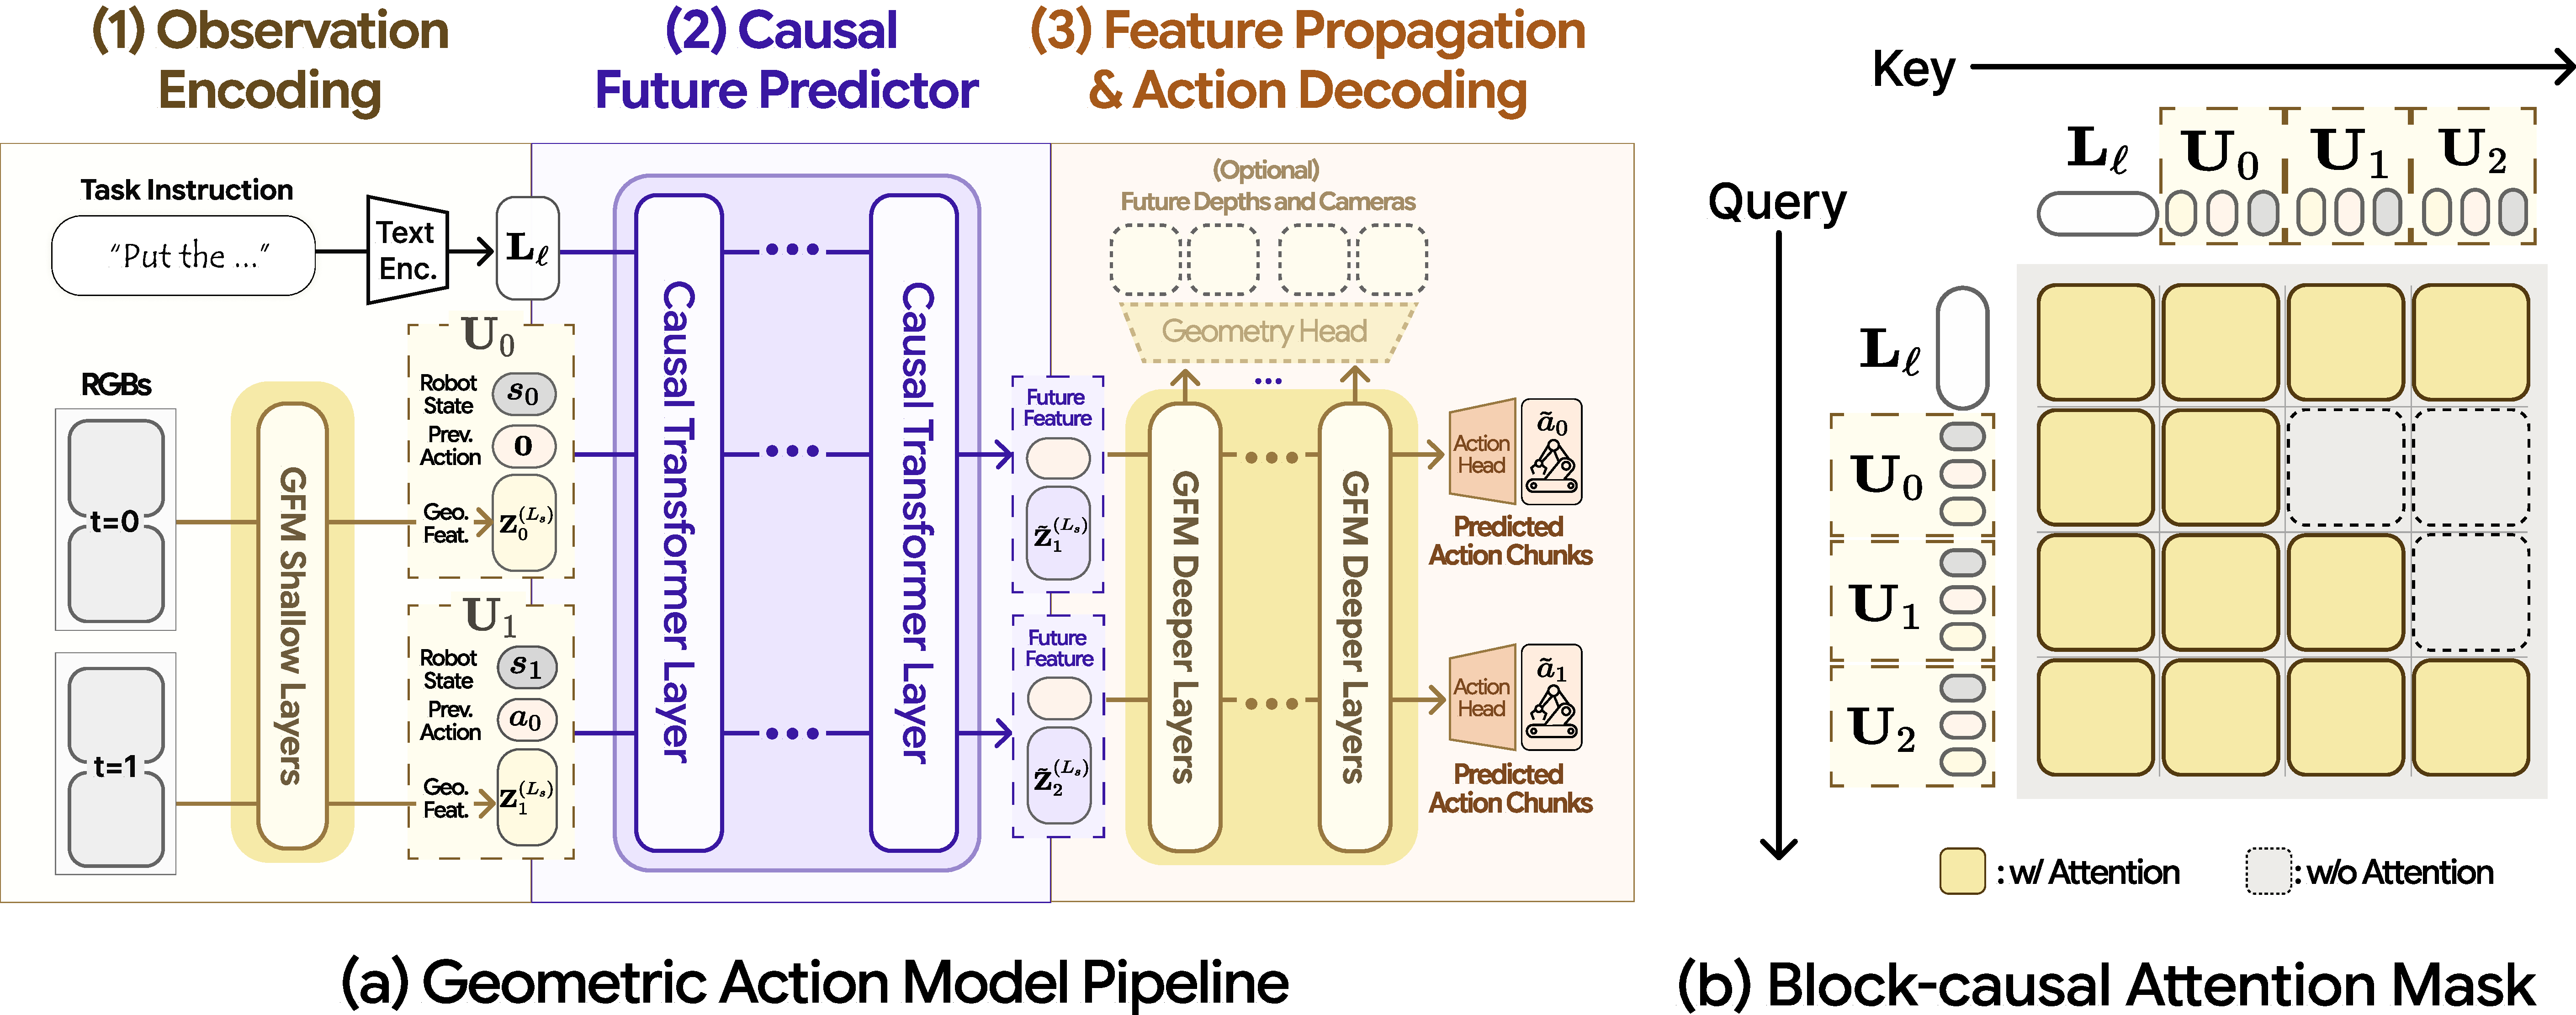
\includegraphics[width=1\linewidth]{figures/arch3.pdf}
  \caption{\textbf{Main architecture of GAM.} }
  \vspace{-15pt}

    \label{fig:arch}
\end{figure}

\noindent\textbf{Problem Formulation.} We consider language-conditioned robot manipulation. At each timestep $t$, the robot receives a multi-view RGB observation $o_t = \{I_{v,t}\}_{v=1}^{V}$ from $V$ fixed cameras, a proprioceptive state $s_t \in \mathbb{R}^{d_s}$ describing the robot's joint configuration and end-effector pose, and a natural-language task instruction $\ell$ that is held constant throughout an episode. The policy $\pi_\theta$ must produce an action chunk $\hat{a}_t \in \mathbb{R}^{C \times d_a}$ of length $C$, encoding the next $C$ delta-pose or joint commands to be executed open-loop before the next observation is acquired. We learn a policy:
\begin{equation}
    \pi_\theta\colon\;\big(\{o_{t-H+1}, \ldots, o_t\},\, \{s_{t-H+1}, \ldots, s_t\},\, \{a_{t-H}, \ldots, a_{t-1}\},\, \ell\big)\;\mapsto\;\hat a_t
\end{equation}
from a dataset of $N$ expert demonstrations $\mathcal{D} = \{(\tau_i, \ell_i)\}_{i=1}^N$, where each trajectory $\tau_i = (o_t, s_t, a_t)_{t=1}^{T_i}$ pairs a sequence of observations, states, and executed action chunks with a fixed instruction $\ell_i$. The policy conditions on a context window of $H$ recent timesteps.


\noindent\textbf{Overview.} In the following sections, we explain how we transform a pretrained GFM into a
language-conditioned world-action model. Our key idea is to split the GFM into two parts and insert a causal temporal predictor between them. This design lets GAM formulate future prediction directly inside the GFM latent space, enabling all predictive computation to be performed in the GFM's geometric representation space.

Concretely, our framework operates in three sequential stages inside the GFM. First, the \textbf{observation encoder} (§\ref{sec:method:encoding}) repurposes the shallow layers of the GFM to extract latent geometric features from multi-view observations. Next, the \textbf{causal future predictor} (§\ref{sec:method:predictor}) operates at the split layer, where it combines these geometric features with language, proprioception, and action history to
predict future latent tokens. Finally, during \textbf{feature propagation and decoding} (§\ref{sec:method:decoding}), the predicted future tokens are routed through the remaining deep GFM blocks to simultaneously decode future geometry and the final action chunk $\hat{a}_t$. Figure~\ref{fig:arch} (a) shows the overall architecture of our model.

\subsection{Observation Encoder}
\label{sec:method:encoding}
We first reuse the shallow layers of the pretrained GFM as the observation encoder. Let $L_s$ denote the split layer where the causal future predictor is inserted. The original GFM transformer stack is then decomposed into an encoder and a decoder:
\begin{equation}
    E_{\leq L_s}
    =
    f^{(L_s)}
    \circ
    \cdots
    \circ
    f^{(1)},
    \qquad
    D_{> L_s}
    =
    f^{(M)}
    \circ
    \cdots
    \circ
    f^{(L_s+1)} .
\end{equation}
Here, the choice of $L_s$ is important because $L_s$ must be deep enough to extract sufficiently rich visual features from the raw observations, yet shallower than the earliest layer used in the DPT head $L_s < m_1$, so that predicted future states can be decoded into future geometries by the DPT heads.

After defining this split layer $L_s$, for each timestep $t'$ in the context window, we tokenize the multi-view RGB observation $o_{t'}=\{I_{v,t'}\}_{v=1}^{V}$ using the original GFM patch embedding. This produces the initial multi-view token sequence:
\begin{equation}
    \mathbf{Z}_{t'}^{(0)}
    =
    \big[
        \mathbf{z}_{1,t'}^{(0)},\ldots,
        \mathbf{z}_{V,t'}^{(0)}
    \big]
    \in
    \mathbb{R}^{V(1+P)\times d},
\end{equation}
where each view contributes one camera token and $P$ patch tokens. The observation encoder maps these tokens to the split-layer representation $\mathbf{Z}_{t'}^{(L_s)}$. By applying this encoding independently to each timestep in the context window, the output of this stage is a sequence of per-timestep geometric latent states $\{\mathbf{Z}_{t-H+1}^{(L_s)},\ldots,\mathbf{Z}_{t}^{(L_s)}\}$.



\subsection{Causal Future Predictor}
\label{sec:method:predictor}

After the observation encoder, GAM performs temporal prediction directly at the split layer $L_s$, forecasting the next latent geometric state from current and past observations while conditioning on the task instruction, proprioception, and action history. To this end, we insert a causal future predictor $g_\phi$ between the shallow encoder $E_{\leq L_s}$ and the deep decoder $D_{>L_s}$.
For each timestep $t'$ in the context window, the encoder provides latent tokens $\mathbf{Z}_{t'}^{(L_s)}$, and we embed the proprioceptive state $s_{t'}$ and previous action $a_{t'-1}$ as tokens:
\begin{equation}
    \mathbf{p}_{t'} = \psi_s(s_{t'}), 
    \qquad
    \mathbf{q}_{t'} = \psi_a(a_{t'-1}),
\end{equation}
with $\psi_s, \psi_a$ lightweight projection layers, and the instruction $\ell$ into language tokens $\mathbf{L}_{\ell}$ with a pretrained text encoder. We then form a per-timestep token block by concatenating the encoded GFM tokens with the proprioception and action-history tokens $\mathbf{U}_{t'}=[\mathbf{p}_{t'};\mathbf{q}_{t'};\mathbf{Z}_{t'}^{(L_s)}]$. The full input to the causal future predictor is $\mathbf{X} = [\mathbf{L}_\ell; \mathbf{U}_{t'-H+1}; \ldots; \mathbf{U}_{t'}]$.

The combined sequence $\mathbf{X}$ is then processed through block-causal self-attention~\citep{wang2025pi}, ensuring the model incorporates past and present contexts without future leakage, as illustrated in Figure~\ref{fig:arch} (b). At the final layer of the predictor $g_\phi$, we read off the predictions from their respective sequence slots. Specifically, the hidden states corresponding to the geometry slots forecast the latent geometric tokens of the future frame, denoted as $\tilde{\mathbf{Z}}_{t'+1}^{(L_s)}$. Concurrently, the hidden state of the designated previous-action slot is projected to produce a predicted next action token $\tilde{\mathbf{a}}_{t'} \in \mathbb{R}^{d}$, in direct analogy to next-token prediction in a causal language model. By jointly forecasting action and geometric latents in this layer, we ensure that action tightly interacts with spatial representations.

This design of introducing a causal transformer predictor $g_\phi$ allows the pretrained GFM to acquire language-conditioned temporal world modeling with \textit{minimal} architectural modification. Only the inserted $g_\phi$ needs to learn how to fuse language, proprioception, and action history with GFM latent features. The resulting predictions, $\widetilde{\mathbf{Z}}_{t'+1}^{(L_s)}$ and $\tilde{\mathbf{a}}_{t'}$, are then passed to the remaining GFM blocks for joint geometry and action decoding.

\subsection{Feature Propagation and Action Decoding}
\label{sec:method:decoding}

Following the causal future predictor, the single action token $\tilde{\mathbf{a}}_{t'}$ is replicated $V$ times to form a set of per-view action tokens $\{\tilde{\mathbf{a}}_{v,t'}\}_{v=1}^{V}$, where $\tilde{\mathbf{a}}_{v,t'} = \tilde{\mathbf{a}}_{t'}$. Concatenated with the geometry tokens, they are fed through the remaining GFM blocks $D_{> L_s}$. We perform this \emph{feature propagation} by appending each view's corresponding action token $\tilde{\mathbf{a}}_{v,t'}$ directly to its geometry token sequence for each timestep:
\begin{equation}
    \tilde{\mathbf{Z}}_{t'+1}^{(M)} = \big(f^{(M)} \circ \cdots \circ f^{(L_s+1)}\big)\!\Big(\Big[\big[\tilde{\mathbf{Z}}_{1,t'+1}^{(L_s)};\, \tilde{\mathbf{a}}_{1,t'}\big], \ldots, \big[\tilde{\mathbf{Z}}_{V,t'+1}^{(L_s)};\, \tilde{\mathbf{a}}_{V,t'}\big]\Big]\Big).
\end{equation}
To prevent future leakage, we extend the predictor's causal mask strategy to the GFM's remaining global attention layers ($f_{\text{global}}^{(m)}$).

Finally, the propagated features are decoded by two heads. The lightweight action head $h_{\text{act}}$ aggregates action tokens over the context window to regress the executable action chunk $\hat a_{t'}$, while the original GFM depth head $h_{\text{depth}}$ decodes geometry tokens into action-aligned future depth maps. The GFM's deep blocks, originally pretrained to decode shallow features into 3D geometry, are thus repurposed here as the decoder of the world model's predicted future.

\subsection{Training and Inference}
\label{sec:method:training}
The policy is trained end-to-end by minimizing a multi-task objective over action execution, world modeling, and geometric decoding:
\begin{equation}
    \mathcal{L}_{\text{total}} = \lambda_{\text{act}} \mathcal{L}_{\text{act}} + \lambda_{\text{feat}} \mathcal{L}_{\text{feat}} + \lambda_{\text{depth}} \mathcal{L}_{\text{depth}},
\end{equation}
where the $\lambda$ factors balance each term and $\mathcal{H} = \{t-H+1, \ldots, t\}$ is the context window. The \emph{action} loss $\mathcal{L}_{\text{act}}$ is an $\ell_1$ regression between the decoded action chunk $\hat a_{t'}$ and the expert action $a_{t'}$ over all $t' \in \mathcal{H}$. The \emph{future-feature} loss $\mathcal{L}_{\text{feat}}$ anchors the predictor $g_\phi$ to temporal geometric transitions by aligning predicted future tokens $\tilde{\mathbf{Z}}_{t'+1}^{(L_s)}$ with the actual next frame $\mathbf{Z}_{t'+1}^{(L_s)}$ extracted from frozen GFM:
\begin{equation}
    \mathcal{L}_{\text{feat}} = \sum_{t' \in \mathcal{H}} \left\| \tilde{\mathbf{Z}}_{t'+1}^{(L_s)} - \mathbf{Z}_{t'+1}^{(L_s)} \right\|_1.
\end{equation}
The \emph{future-depth} loss $\mathcal{L}_{\text{depth}}$ grounds the predicted future in valid 3D structure by supervising the decoded depth $\tilde{D}_{t'+1}=h_{\text{depth}}(\tilde{\mathbf{Z}}_{t'+1}^{(m^*)})$ using depth head $h_{\text{depth}}$ against ground-truth future depth $D_{t'+1}$, adopting the scale-invariant and gradient-matching penalties of the GFM~\citep{lin2025depth, wang2026vggt}. 

At inference, we maintain the historical context online with key-value caching, so each step processes only the new observation $o_t$ and previous action $a_{t-1}$ in a single feed-forward pass. 